En este capítulo se describirá el diseño de la red de la empresa, incluyendo la topología,
la infraestructura de red, los dispositivos de red que se van a utilizar y las tecnologías implementadas.

\section{Diseño de red}
Para interconectar las sedes de la empresa se ha optado por una topología en estrella
porque se centraliza la gestión en un nodo central (oficina central). Además, el pliego de proyectos \footnote{\href{https://contrataciondelestado.es/wps/wcm/connect/PLACE_es/Site/area/docAccCmpnt?srv=cmpnt&cmpntname=GetDocumentsById&source=library&DocumentIdParam=10e9102e-09a6-42de-810d-d08c7c77bd65}{\texttt{Pliego de prescripciones técnicas para la contratación de servicios de telecomunicaciones de voz, fijas y móviles, red de acceso de datos,
			intranet e internet para el Consorcio de Aguas de la Zona Gaditana}}} especifica que \textit{``accederán a internet através del circuito ubicado al efecto en la Sede Principal''}, por lo que el acceso a Internet será unicamente en este punto, simplificando así la administración y el mantenimiento de la red. Además, permite que sea escalable, ya que se pueden agregar más edificios sin tener que reconfigurar toda la red. Esta estructura facilita redundancia en el núcleo y reduce costos al evitar conexiones complejas. En la Figura~\ref{fig:interconexion} se puede observar una representación gráfica de la topología en estrella de las instalaciones de la empresa.

\vspace{0.5cm}
Como tecnología principal de interconexión entre las sedes se ha optado por SD-WAN (Software Defined Wide Area Network) ya que permite una gestión centralizada, mayor flexibilidad, seguridad avanzada y facilita la integración de múltiples sedes e integración en tiempo real sin interrupciones. Esta tecnología es ideal para empresas que necesitan conectar varias ubicaciones de manera eficiente, segura y con capacidad de adaptación a diferentes proveedores y tipos de acceso.
Además, permite priorizar el tráfico crítico, aplicar políticas de seguridad de forma centralizada y simplificar
la administración de la red.

\vspace{0.5cm}
Para la interconexión de las sedes se han estudiado varios proveedores de servicios de telecomunicaciones, como Vodafone, Orange y Telefónica. Para este proyecto se ha optado por Vodafone como principal operador por su mejor oferta de servicios, precios y por ajustarse a las necesidades de la red. Vodafone ofrece un servicio de SD-WAN de Cisco Meraki que permite la creación de redes privadas virtuales (VPN), proporciona una mayor seguridad y control sobre el tráfico de datos, y facilita la gestión centralizada de la red. En la Tabla~\ref{tab:proveedores_red} se puede observar los proveedores de servicios de telecomunicaciones estudiados y las características principales de cada uno.

\begin{figure}[H]
	\centering
	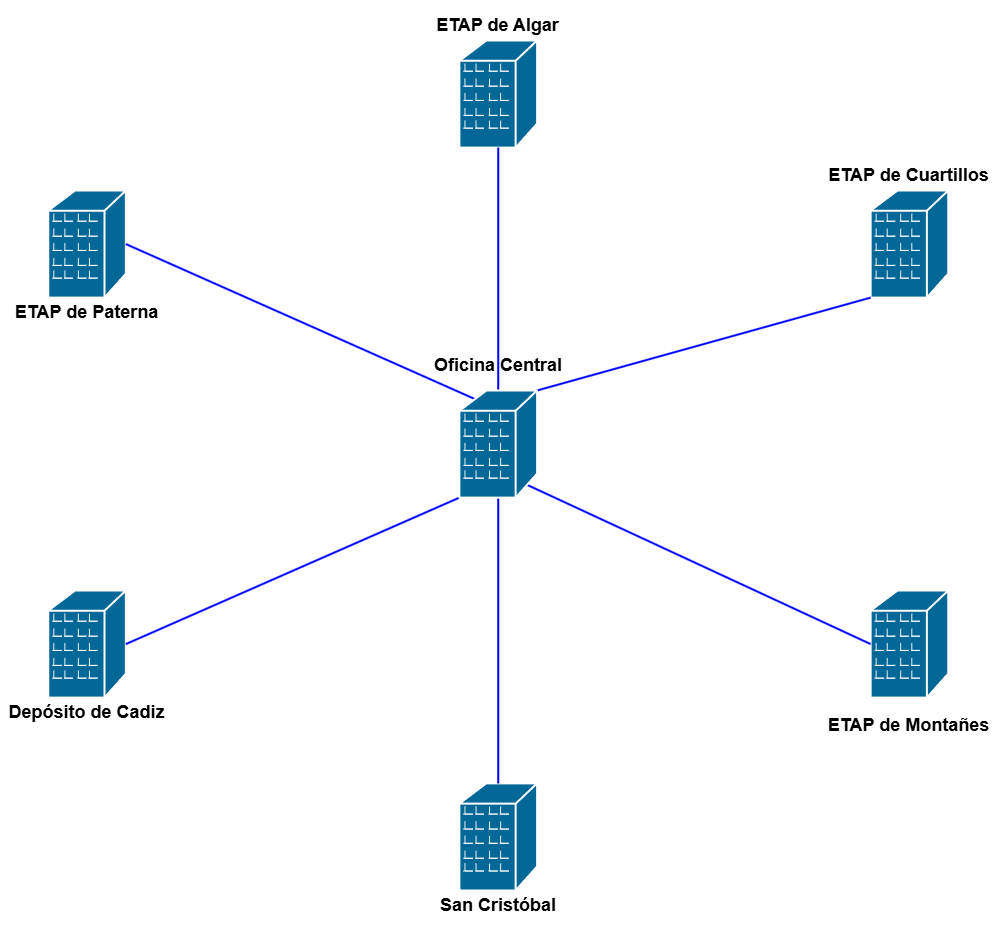
\includegraphics[width=0.7\textwidth]{images/Esquema_interconexion_sedes.png}
	\caption{Esquema de interconexión de sedes}
	\label{fig:interconexion}
\end{figure}

\begin{table}[htb]
	\centering
	\resizebox{\textwidth}{!}{%
		\begin{scriptsize}
			\begin{tabular}{|l|p{2.8cm}|p{3.3cm}|p{4cm}|c|}
				\hline
				\textbf{Proveedor} & \textbf{Tecnología principal} & \textbf{Seguridad y gestión}                                   & \textbf{Ventajas destacadas}                                               & \textbf{Precio/mes/sede}         \\
				                   &                               &                                                                &                                                                            & \footnotesize{(IVA no incluido)} \\ \hline
				Orange             & VPN, FTTH                     & Soluciones de seguridad integrales en la nube.                 & Red privada y unificada, acceso sencillo a recursos compartidos.           & 50\,€                            \\ \hline
				Telefónica         & SD-WAN (Cisco Meraki), MPLS   & Firewall avanzado y control de accesos, detección de amenazas. & Integración con Cisco Meraki y gestión centralizada sin inversión inicial. & 75\,€                            \\ \hline
				Vodafone           & SD-WAN (Cisco Meraki), VPN    & Firewall de última generación y gestión centralizada.          & Visualización avanzada del tráfico y conectividad mejorada entre sedes.    & 64\,€                            \\ \hline
			\end{tabular}
		\end{scriptsize}
	}
	\caption{Comparativa de proveedores de servicios de telecomunicaciones}
	\label{tab:proveedores_red}
\end{table}

Por otro lado, se pide para algunas sedes (no se especifica cuáles), un caudal de respaldo obligatorio que tiene que ir montado sobre distinta infraestructura o aplicando tecnologías diferentes o distinto operador. Para ello, se va a optar por Telefónica utilizando también su servicio SD-WAN de Cisco Meraki. Además, se pide que se tenga un un dispositivo independiente y distinto al principal para el enlace de respaldo, para esto, contará con un dispositivo diferente configurado en modo \textit{Warm Spare (HA)} \cite{meraki_warm_spare}, lo que garantiza la continuidad del servicio mediante un segundo equipo en espera, preparado para asumir el control en caso de que el principal falle. También, la funcionalidad de SD-WAN inteligente de Meraki permitirá balancear el tráfico entre el enlace principal y el enlace de respaldo (en este caso, la solución flexWAN de Telefónica), seleccionando dinámicamente el mejor camino según la calidad del enlace y las políticas definidas, asegurando así la redundancia de red y alta disponibilidad

\subsection{Diseño estructural}
La arquitectura de red se ha diseñado siguiendo un modelo jerárquico de tres capas: núcleo, distribución y acceso. Esta jerarquía permite una mejor gestión del tráfico, escalabilidad y redundancia en la red.
\begin{itemize}
	\item \textbf{Capa de núcleo:} se encarga de la interconexión entre las diferentes sedes y la oficina central. Se utilizan dispositivos de alto rendimiento para garantizar una alta disponibilidad y baja latencia en la comunicación entre sedes.
	\item \textbf{Capa de distribución:} se encuentran los dispositivos que conectan los diferentes segmentos de la red, como switches y routers. Se encargan de la gestión del tráfico y la seguridad de la red.
	\item \textbf{Capa de acceso:} se conectan los hosts finales, como ordenadores, impresoras y teléfonos IP. Se utilizan switches de acceso para conectarlos a la red.
\end{itemize}

En la Figura~\ref{fig:diseño_vertical_red} se puede observar el cableado vertical de alguna de las sedes de la empresa.
Esta se encarga de conectar las diferentes plantas de un edificio, permitiendo la interconexión entre los armarios de comunicaciones de cada piso y asegurando la continuidad de la red a lo largo de toda la estructura vertical del edificio. ETAP Cuartillos y ETAP Montañés tienen una organización similar entre ellas y, por otro lado, ETAP Paterna, ETAP Algar y el Depósito de Cádiz comparten una configuración parecida entre sí. La oficina central presenta una estructura diferente al resto, ya que alberga los diferentes servidores de la empresa y la DMZ (zona desmilitarizada) donde se alojan los servidores de la empresa.

\begin{figure}[H]
	\centering
	\includegraphics[width=1\textwidth]{images/diseño_vertical_sedes.png}
	\caption{Diseño vertical de la red}
	\label{fig:diseño_vertical_red}
\end{figure}

En el esquema de red de la Figura~\ref{fig:diseño_vertical_red}, las líneas rojas indican el núcleo de la infraestructura, donde se ubican los dispositivos core y de distribución que manejan el tráfico principal entre sedes. Las líneas naranjas corresponden a la zona de distribución, conectando los equipos de distribución con los de acceso. Por su parte, las líneas amarillas representan la capa de acceso, donde se integran los dispositivos finales. Los círculos en tonos celeste pastel y lila identifican las VLAN de datos y voz, respectivamente, mientras que en la oficina central, el área marcada con un recuadro amarillo indica la DMZ, donde se alojan los servidores corporativos. Para el cableado, se empleará fibra óptica monomodo en los enlaces principales entre los equipos de core y distribución, así como en los tramos verticales entre plantas, garantizando así alta velocidad y baja latencia. En la capa de acceso y para la conexión de los equipos finales, se utilizará cableado estructurado de cobre categoría 6A (Cat 6A), adecuado para velocidades de hasta 10 Gbps dentro de edificios.

\vspace{0.5cm}
En la Figura~\ref{fig:diseño_general} se puede observar el diseño general de la red de la empresa, donde se muestra la interconexión entre las diferentes sedes y la oficina central. Este diseño general permite visualizar cómo se conectan todas las instalaciones de la empresa, formando una red corporativa unificada que facilita la gestión centralizada y la comunicación entre todas las sedes.

\begin{figure}[htb]
	\centering
	\includegraphics[width=1\textwidth]{images/diseño_general.png}
	\caption{Diseño representativo de la red de la empresa}
	\label{fig:diseño_general}
\end{figure}

\subsection{Dispositivos de red}
\label{subsubsec:dispositivos_red}
En esta sección se detallan los equipos de red elegidos para poner en marcha la infraestructura de comunicaciones de
a empresa. Aunque Vodafone no especifica detalladamente los modelos que se entrega a sus clientes, sí se especifica que su solución SD-WAN está basada en la tecnología Cisco Meraki.

% Aunque algunos dispositivos, como los routers o firewalls, suelen ser facilitados por el proveedor de
% telecomunicaciones, en este caso no se cuenta con información precisa sobre los modelos que serán entregados. Por ello,
% se ha optado por seleccionar ejemplos representativos que cumplen con las características técnicas y operativas
% requeridas para el diseño planteado.

% \subsubsection{Dispositivos SW-WAN (Cisco Meraki)}
% Como Vodafone como trabaja con la tecnología SD-WAN de Cisco Meraki se ha optado por realizar una estimación técnica realista de los dispositivos que se usaran. En este caso, se usara equipamiento UTM (Unified Threat Management) que es aquel que tiene múltiples funciones como firewall, VPN, detección de intrusiones y filtrado de contenido. Estos dispositivos proporcionan una solución integral para la seguridad de la red y son ideales para empresas que buscan simplificar su infraestructura de seguridad. 

\subsubsection{Dispositivos de interconexión}
Dado que el proveedor de servicios elegido es Vodafone, el cual ofrece soluciones de conectividad basadas en la tecnología SD-WAN de Cisco Meraki, se ha optado por realizar una estimación técnica realista de los dispositivos que podrían instalarse en cada sede.

\newpage

\vspace{0.5cm}
En este proyecto se propone el uso de dispositivos de la gama Cisco Meraki MX, los cuales son \textit{appliances} de red de tipo UTM (Unified Threat Management). Estos dispositivos combinan en un solo equipo funciones avanzadas de enrutamiento, cortafuegos de nueva generación, conectividad VPN automática (AutoVPN), detección y prevención de intrusiones (IDS/IPS), así como filtrado de contenido.

% \vspace{0.5cm}
%
% Su integración en la arquitectura SD-WAN permite una gestión centralizada desde la nube (Meraki Dashboard), así como la aplicación de políticas de red, seguridad y calidad de servicio de forma unificada. Este tipo de equipamiento resulta especialmente adecuado para entornos distribuidos como el de este proyecto, ya que permite simplificar la infraestructura, mejorar la seguridad y facilitar la escalabilidad de la red.

\vspace{0.5cm}
En la Tabla~\ref{tab:justificacion_meraki} se presenta una justificación técnica de los dispositivos Cisco Meraki MX~\footnote{\href{https://meraki.cisco.com/lib/pdf/meraki_datasheet_mx_es.pdf}{\texttt{Ficha técnica de los Meraki MX}}} propuestos para cada sede del Consorcio de Aguas de la Zona Gaditana. Se ha seleccionado un modelo específico para cada sede, teniendo en cuenta el tamaño y las necesidades de conectividad de cada una.

\begin{table}[H]
	\centering
	\resizebox{\textwidth}{!}{%
		\begin{scriptsize}
			\begin{tabular}{|c|c|p{6cm}|c|}
				\hline
				\textbf{Sede}   & \textbf{Modelo propuesto} & \textbf{Justificación}                                                                                                                                                                                                                                                                              & \textbf{Precio estimado (€)} \\ \hline
				Oficina Central & MX95                      & Nodo central de la red SD-WAN. Actúa como concentrador VPN y punto de salida único a Internet. Requiere alto rendimiento y escalabilidad.                                                                                                                                                           & 3.700                        \\ \cline{2-4}
				                & MX85                      & Será el dispositivo secundario (redundancia) que estará preparado (Warm Spare) en caso de que el principal falle.                                                                                                                                                                                   & 2.130                        \\ \hline
				San Cristóbal   & MX68                      & Sede mediana. El modelo permite hasta 50 usuarios y ofrece margen de crecimiento. Adecuado para cargas medias y conexiones VPN estables.                                                                                                                                                            & 650                          \\ \hline
				\multirow{5}{*}{\begin{tabular}[c]{@{}c@{}}ETAP de Cuartillos\\ ETAP de Montañés\\ ETAP de Paterna\\ ETAP de Algar\\ Depósito de Cádiz\end{tabular}}
				                & \multirow{5}{*}{MX67}     & Sedes pequeñas con necesidades similares de conectividad y escalabilidad. El modelo MX67 es compacto, económico y soporta hasta 50 usuarios, ofreciendo suficientes puertos LAN y funcionalidades para entornos de bajo o moderado tráfico, manteniendo un buen balance entre coste y prestaciones. & \multirow{5}{*}{420}         \\ \hline
			\end{tabular}
		\end{scriptsize}
	}
	\caption{Justificación técnica de los dispositivos Cisco Meraki MX por sede}
	\label{tab:justificacion_meraki}
\end{table}

\noindent
Los modelos seleccionados de la serie Meraki MX  ofrecen las siguientes características:
\begin{itemize}
	\item \textbf{Rendimiento y escalabilidad:} estos modelos están diseñados para manejar cargas de trabajo medianas a altas, con capacidades de procesamiento y memoria adecuadas para soportar múltiples conexiones VPN y tráfico de red.
	\item \textbf{Seguridad avanzada:} todos los modelos incluyen funcionalidades de seguridad integradas, como firewall de nueva generación, detección y prevención de intrusiones (IDS/IPS), filtrado de contenido y protección contra malware, lo que garantiza una defensa robusta contra amenazas cibernéticas.
	\item \textbf{Conectividad VPN:} establecen automáticamente túneles VPN sitio a sitio con conectividad con IPsec
	\item \textbf{Gestión centralizada:} todos los dispositivos se gestionan a través del Meraki Dashboard, que es una plataforma en la nube de Meraki que permite la administración centralizada de la red, la monitorización del rendimiento y la aplicación de políticas de seguridad y calidad de servicio de forma unificada.
	\item \textbf{Facilidad de implementación:} los dispositivos Meraki son conocidos por su facilidad de instalación y configuración, lo que reduce el tiempo y los recursos necesarios para poner en marcha la red.
\end{itemize}

\subsubsection{Switches}
El Consorcio de Aguas de la Zona Gaditana cuenta con siete sedes distribuidas por la provincia de Cádiz.
En la Tabla~\ref{tab:sedes_puertos_acceso} se detalla el número mínimo de puntos de acceso requeridos
para cada sede. Considerando que cada trabajador necesita un ordenador y un teléfono IP, se ha
duplicado el número de puertos solicitados. Además, se ha implementado un margen de crecimiento
del 20\% para permitir futuras ampliaciones de la infraestructura de red.

\begin{table}[H]
	\centering
	\small
	\begin{tabular}{|l|l|l|l|l|}
		\hline
		\textbf{Denominación de la sede} & \textbf{Nº de puertos mínimo} & \textbf{Nº de puertos con escalabilidad} \\ \hline
		Oficina central                  & 30                            & 72                                       \\ \hline
		San Cristóbal                    & 15 + 5 + 5                    & 36 + 12 + 12                             \\ \hline
		ETAP de Cuartillos               & 5 + 5                         & 12 + 12                                  \\ \hline
		ETAP de Montañés                 & 5 + 5                         & 12 + 12                                  \\ \hline
		ETAP de Paterna                  & 5                             & 12                                       \\ \hline
		ETAP de Algar                    & 5                             & 12                                       \\ \hline
		Depósito de Cádiz                & 5                             & 12                                       \\ \hline
	\end{tabular}
	\caption{Número de puertos de acceso a la red}
	\label{tab:sedes_puertos_acceso}
\end{table}

Se han comparado diferentes modelos de switches por fabricante según las necesidades de cada sede (ver Tabla~\ref{tab:switches}). Finalmente, se seleccionan dispositivos Cisco por su relación calidad-precio: el Catalyst 9300-24P \cite{cisco_9300_24p_e_shop, cisco_9300_24p_e_datasheet} para la Oficina Central y San Cristóbal, el Catalyst 3560-CX-12PD-S \cite{cisco_3560_cx_12pd_s_shop, cisco_3560_cx_12pd_s_datasheet} para el resto de sedes, y el WS-C2960L-16TS-LL \cite{cisco_2960l_16ts_ll_datasheet} como switch de acceso en todos los edificios.

\renewcommand{\arraystretch}{1.2} % Puedes ajustar el valor (1.2, 1.3, 1.5, etc.). Esto es para aumentar el espacio entre filas
\begin{table}[H]
	\centering
	\small
	\resizebox{\textwidth}{!}{%
		\begin{tabular}{|c|c|c|c|c|}
			\hline
			\textbf{Fabricante} & \textbf{Rol} & \textbf{Modelo}         & \textbf{Sedes que lo necesitan}          & \textbf{Precio/unidad} \\ \hline
			Cisco               & Distribución & Catalyst 9300-24P       & Oficina Central, San Cristóbal           & 1.160€                 \\ \cline{3-5}
			                    &              & Catalyst 3560-CX-12PD-S & ETAP Cuartillos, ETAP Montañés,          & 1.120€                 \\
			                    &              &                         & ETAP Paterna, ETAP Algar, Depósito Cádiz &                        \\ \cline{2-5}
			                    & Acceso       & WS-C2960L-16TS-LL       & Oficina Central (5), San Cristóbal (4)   & 410€                   \\
			                    &              &                         & ETAP Cuartillos (2), ETAP Montañés (2)   &                        \\
			                    &              &                         & ETAP Paterna, ETAP Algar, Depósito Cádiz &                        \\ \hline

			Juniper             & Distribución & EX4300-24P              & Oficina Central, San Cristóbal           & 2.900€                 \\ \cline{3-5}
			                    &              & EX2300-C-12P            & ETAP Cuartillos, ETAP Montañés,          & 700€                   \\
			                    &              &                         & ETAP Paterna, ETAP Algar, Depósito Cádiz &                        \\ \cline{2-5}
			                    & Acceso       & EX2300-C-12P            & Oficina Central (6), San Cristóbal (5)   & 700€                   \\
			                    &              &                         & ETAP Cuartillos (2), ETAP Montañés (2),  &                        \\
			                    &              &                         & ETAP Paterna, ETAP Algar, Depósito Cádiz &                        \\ \hline

			Huawei              & Distribución & S5720-28X-PWR-SI-AC     & Oficina Central, San Cristóbal           & 1.030€                 \\ \cline{3-5}
			                    &              & S5720-14X-PWH-SI-AC     & ETAP Cuartillos, ETAP Montañés,          & 700€                   \\
			                    &              &                         & ETAP Paterna, ETAP Algar, Depósito Cádiz &                        \\ \cline{2-5}
			                    & Acceso       & S5720-28X-PWR-LI-AC     & Oficina Central (3), San Cristóbal (4)   & 360€                   \\
			                    &              &                         & ETAP Cuartillos (2), ETAP Montañés (2),  &                        \\
			                    &              &                         & ETAP Paterna, ETAP Algar, Depósito Cádiz &                        \\ \hline
		\end{tabular}%
	}
	\caption{Comparativa de switches por fabricante y sedes según necesidades.}
	\begin{tcolorbox}[colback=gray!10!white, colframe=gray!70!black, title=NOTA:, size=title]
		\textit{El número reflejado en cada paréntesis indica la cantidad de dispositivos de ese tipo en las sedes mencionadas}
	\end{tcolorbox}
	\label{tab:switches}
\end{table}
\renewcommand{\arraystretch}{1} % Restablecer el valor por defecto

\subsubsection{Firewall}
Siguiendo las especificaciones técnicas descritas en la sección~\ref{subsec:especificaciones_tecnicas_firewall}, y teniendo en cuenta que Vodafone trabaja con dispositivos de la marca Fortinet, se ha seleccionado el modelo \texttt{Fortinet FortiGate FG-100F-HA} como solución de seguridad perimetral para la sede central.

\vspace{0.5cm}
Este firewall de próxima generación proporciona un conjunto completo de funcionalidades de protección, incluyendo prevención de intrusiones, inspección profunda de paquetes (DPI), control de aplicaciones, filtrado web y antivirus. Su integración permite reforzar la seguridad del perímetro WAN y complementar las funciones básicas de firewall ya incluidas en los dispositivos Cisco Meraki MX utilizados en la red SD-WAN.

\vspace{0.5cm}
El modelo FG-100F-HA permite configuraciones en alta disponibilidad (HA), soporta múltiples interfaces de red de alta velocidad y está diseñado para entornos empresariales de tráfico medio-alto, como es el caso de la oficina central que actúa como nodo concentrador del tráfico de todas las sedes.

\vspace{0.5cm}
Esta solución permite reforzar la seguridad global de la red, especialmente en el punto crítico donde se concentra todo el tráfico proveniente de las sedes remotas. El FortiGate actúa como firewall perimetral, mientras que el \textit{appliance} Cisco Meraki MX250 se encarga de la conectividad SD-WAN, aunque tiene firewall integrado pero no suficiente para esta red de la empresa, estos se complementan entre sí para proporcionar una solución de seguridad robusta y escalable.

\subsubsection{Telefonía IP}
En cuanto a la telefonía IP, se ha optado por teléfonos que cumplan con los requisitos que se comentan en la sección \ref{sec:requisitos_telefonia_ip}. En la Tabla~\ref{tab:telefonos_ip} se muestran algunos modelos que cumplen con los requisitos necesarios que pide el pliego de proyectos.
\begin{table}[H]
	\centering
	\small
	\begin{tabular}{|c|c|c|p{6.5cm}|}
		\hline
		\textbf{Fabricante} & \textbf{Modelo} & \textbf{Precio aprox.} & \textbf{Características principales}                                                                                                               \\ \hline
		Grandstream         & GRP2602G        & 37€                    & 2 lineas y 4 cuentas SIP, puertos Gigabit con PoE integrado, pantalla LCD, manos libres Full-Duplex, audio HD, EHS                                 \\ \hline
		Grandstream         & GRP2612G        & 45€                    & 4 lineas multiuso y 4 cuentas SIP, dobles puertos GE a 10/100/1000 Mbps con PoE integrada, audio HD (Noise Shield), Wi-Fi de doble banda integrado \\ \hline
		Yealink             & SIP-T31G        & 55€                    & 2 cuentas VoIP, pantalla LCD, doble puerto Gigabit Ethernet, manos libre Full-Duplex, soporte IPv6, EHS                                            \\ \hline
		Fanvil              & X3SP Pro        & 65€                    & 4 líneas SIP, Auriculares inalámbricos EHS, Puertos rápidos duales, PoE integrado, Full-Duplex (AEC)                                               \\ \hline
	\end{tabular}
	\caption{Comparativa de Teléfonos IP}
	\label{tab:telefonos_ip}
\end{table}

Se va a optar por el modelo \texttt{Grandstream GRP2612G} \cite{grandstream_grp2612_datasheet} para toda la empresa, ya que es un modelo que cumple con los requisitos técnicos necesarios y es compatible con la solución de telefonía en la nube.

\subsubsection{Resumen de los dispositivos de red}
En la Tabla~\ref{tab:dispositivos_red} se presenta un resumen de los dispositivos de red seleccionados para el Consorcio de Aguas de la Zona Gaditana.

\begin{table}[H]
	\centering
	\small
	\resizebox{\textwidth}{!}{%
		\begin{tabular}{|c|c|c|c|c|}
			\hline
			\textbf{Dispositivo}                          & \textbf{Modelo}         & \textbf{Cantidad} & \textbf{Precio/unidad} & \textbf{Precio total} \\ \hline
			Dispositivo SD-WAN                            & Cisco Meraki MX95       & 1                 & 3.700€                 & 3.700€                \\ \hline
			Dispositivo SD-WAN                            & Cisco Meraki MX85       & 1                 & 2.130€                 & 2.130€                \\ \hline
			Dispositivo SD-WAN                            & Cisco Meraki MX68       & 1                 & 650€                   & 650€                  \\ \hline
			Dispositivo SD-WAN                            & Cisco Meraki MX67       & 5                 & 420€                   & 2.100€                \\ \hline
			Switch de distribución                        & Catalyst 9300-24P       & 2                 & 1.160€                 & 2.320€                \\ \hline
			Switch de distribución                        & Catalyst 3560-CX-12PD-S & 5                 & 1.120€                 & 5.600€                \\ \hline
			Switch de acceso                              & WS-C2960L-16TS-LL       & 16                & 410€                   & 6.560€                \\ \hline
			Firewall                                      & FortiGate FG-100F-HA    & 1                 & 1800€                  & 1.800€                \\ \hline
			Teléfono IP                                   & Grandstream GRP2612G    & 38                & 45€                    & 1.710€                \\ \hline
			\hline
			\multicolumn{4}{|c|}{\textbf{Total estimado}} & \textbf{26.570€}                                                                             \\ \hline
		\end{tabular}
	}
	\caption{Resumen de dispositivos de red seleccionados}
	\label{tab:dispositivos_red}
\end{table}

\subsection{Servicios de red necesarios}
En este proyecto no se implementarán directamente todos los servicios de red, ya que el objetivo es realizar un diseño de red adaptado a las necesidades tomadas de referencia del pliego del Consorcio de Aguas de la Zona Gaditana. A continuación, se describen los servicios de red que se consideran necesarios para el correcto funcionamiento de la infraestructura de comunicaciones de la empresa, tal y como se recoge en la Tabla~\ref{tab:servicios-red}. Estos servicios son fundamentales para garantizar la conectividad, la seguridad y la gestión eficiente de la red.

\begin{table}[H]
	\centering
	\small
	\resizebox{\textwidth}{!}{%
		\begin{tabular}{|p{4cm}|p{6.5cm}|p{5.5cm}|}
			\hline
			\textbf{Servicio}                      & \textbf{Descripción}                                              & \textbf{Observaciones}                                                     \\ \hline
			Red Privada Virtual (VPN)              & Conectividad segura entre todas las sedes                         & Nodo central (Oficina Central) como HUB + VPN Site-to-Site para cada sede. \\ \hline
			Active Directory (AD)                  & Gestión centralizada de usuarios, políticas y accesos.            & Servidor virtualizado en Oficina Central.                                  \\ \hline
			DNS interno                            & Resolución de nombres para servicios internos.                    & Integrado con el AD en la Oficina Central.                                 \\ \hline
			DHCP                                   & Asignación dinámica de IP por sede.                               & Centralizado en Oficina Central + DHCP Relay en cada sede.                 \\ \hline
			Centralita VoIP en la nube             & Telefonía fija integrada                                          & Con terminales IP en cada sede.                                            \\ \hline
			Correo electrónico corporativo         & Gestión de cuentas de correo, buzones compartidos y seguridad.    & Solución cloud (Microsoft 365).                                            \\ \hline
			Web corporativa                        & Sitio web institucional accesible públicamente.                   & Alojamiento en la nube.                                                    \\ \hline
			Cortafuegos de nueva generación (NGFW) & Seguridad perimetral, visibilidad del tráfico, control de acceso. & Instalado en la Oficina Central como único punto de acceso a Internet.     \\ \hline
			Backup en la nube                      & Copias de seguridad de sistemas físicos y virtuales.              & Almacenamiento en la nube.                                                 \\ \hline
			Acceso a Internet                      & Salida a Internet centralizada desde la Oficina Central           & A través del firewall central en la Oficina Central.                       \\ \hline
		\end{tabular}
	}
	\caption{Resumen de servicios de red necesarios}
	\label{tab:servicios-red}
\end{table}

\section{Esquema de direccionamiento}
Para abordar el problema del agotamiento de direcciones, se ha diseñado un esquema en IPv6. Cada sede dispone de dos VLANs principales, una para datos con ID 10 y otra para voz con ID 20, lo que permite segmentar el tráfico y mejorar la seguridad y el rendimiento de la red. Además, la Oficina Central incluye una VLAN DMZ con ID 30 para los servidores que deben ser accesibles desde Internet. Cada sede tendrá asignado un bloque de direcciones IPv6 /56, lo que permite crear hasta 256 subredes /64 dentro de cada sede, una para cada VLAN. Esto proporciona una gran flexibilidad y escalabilidad para futuras expansiones de la red, ya que cada VLAN puede crecer independientemente sin necesidad de reconfigurar la red completa.

\vspace{0.5cm}
Se asume que el ISP asigna el bloque \texttt{2001:db8:1234::/48}. A partir de este bloque, se han reservado subredes /64 para cada VLAN de cada localización. Además, todas las direcciones IP se asignarán mediante un servidor DHCP (Dynamic Host Configuration Protocol), que proporcionará las direcciones dentro de los rangos definidos en la Tabla~\ref{tab:esquema_ipv6_dhcp}, evitando conflictos de direcciones en la red. El servidor DHCP estará centralizado en la Oficina Central, y cada router de delegación actuará como relay DHCP para reenviar las solicitudes de los dispositivos de su ubicación al servidor central. De este modo, se garantiza que cada oficina reciba direcciones IP dentro de su rango específico, sin solapamientos entre instalaciones ni VLANs. En la DMZ, las IPs serán asignadas de forma estática.

\begin{table}[H]
	\centering
	\resizebox{\textwidth}{!}{%
		\begin{tabular}{|c|c|c|c|c|}
			\hline
			\textbf{Sede}     & \textbf{Prefijo de sede} & \textbf{VLAN} & \textbf{Dir. de Red} & \textbf{Máscara} \\
			\hline
			Oficina central   & 2001:db8:1234:0100::/56  & Datos         & 2001:db8:1234:0100:: & /64              \\ \cline{3-5}
			                  &                          & Voz           & 2001:db8:1234:0101:: & /64              \\ \cline{3-5}
			                  &                          & DMZ           & 2001:db8:1234:0102:: & /64              \\ \hline
			San Cristóbal     & 2001:db8:1234:0200::/56  & Datos         & 2001:db8:1234:0200:: & /64              \\ \cline{3-5}
			                  &                          & Voz           & 2001:db8:1234:0201:: & /64              \\ \hline
			ETAP Cuartillos   & 2001:db8:1234:0300::/56  & Datos         & 2001:db8:1234:0300:: & /64              \\ \cline{3-5}
			                  &                          & Voz           & 2001:db8:1234:0301:: & /64              \\ \hline
			ETAP Montañés     & 2001:db8:1234:0400::/56  & Datos         & 2001:db8:1234:0400:: & /64              \\ \cline{3-5}
			                  &                          & Voz           & 2001:db8:1234:0401:: & /64              \\ \hline
			ETAP Paterna      & 2001:db8:1234:0500::/56  & Datos         & 2001:db8:1234:0500:: & /64              \\ \cline{3-5}
			                  &                          & Voz           & 2001:db8:1234:0501:: & /64              \\ \hline
			ETAP Algar        & 2001:db8:1234:0600::/56  & Datos         & 2001:db8:1234:0600:: & /64              \\ \cline{3-5}
			                  &                          & Voz           & 2001:db8:1234:0601:: & /64              \\ \hline
			Depósito de Cádiz & 2001:db8:1234:0700::/56  & Datos         & 2001:db8:1234:0700:: & /64              \\ \cline{3-5}
			                  &                          & Voz           & 2001:db8:1234:0701:: & /64              \\ \hline
		\end{tabular}
	}
	\caption{Esquema de direccionamiento IPv6 para todas las sedes}
	\label{tab:esquema_ipv6_dhcp}
\end{table}

\section{Seguridad y firewall}
En esta sección se abordarán los aspectos de seguridad de la red, incluyendo la plataforma de seguridad
a utilizar y las reglas del firewall. Cabe recalcar que no se implementarán los servicios de seguridad por
el poco tiempo que se tiene para realizar el proyecto.

\subsection{Plataforma de seguridad}
Como plataforma de firewall de nueva generación se ha seleccionado el \texttt{FortiGate Next-Generation Firewall (NGFW)} \cite{ngfw_fortinet}, que están diseñados para ofrecer seguridad avanzada en cualquier entorno (on-premise, nube, remoto). Además, FortiGate es el firewall que utiliza Vodafone en sus redes, lo que garantiza una integración fluida con los servicios de telecomunicaciones de la empresa. También, es el cortafuegos más implementado, con más del 50\% de la participación en el mercado global.

\vspace{0.5cm}
Por otro lado, la plataforma de respuesta ante incidentes se basará en \texttt{Microsoft Sentinel} \cite{microsoft_sentinel_overview}, que es un servicio de SIEM (*Security Information and Event Management*) y SOAR (*Security Orchestration, Automation, and Response*) en la nube. \texttt{Microsoft Sentinel} permite la recopilación, análisis y correlación de datos de seguridad de toda la infraestructura, facilitando la detección y respuesta ante amenazas.


\subsection{Reglas firewall}
La Oficina Central de la empresa contará con un esquema de seguridad perimetral para proteger la red, incluyendo una zona desmilitarizada (DMZ). Todas las sedes remotas accederán a Internet a través de la Oficina Central,
por lo que el firewall de esta sede será el punto de control de acceso a Internet para toda la organización. A continuación se describen algunas reglas básicas de seguridad que que tendrá el firewall de la Oficina Central:

\begin{table}[H]
	\centering
	\resizebox{\textwidth}{!}{%
		\begin{tabular}{|c|c|c|c|c|c|c|}
			\hline
			\textbf{Regla} & \textbf{Acción} & \textbf{IP Origen} & \textbf{IP Destino} & \textbf{Protocolo} & \textbf{Puerto Origen} & \textbf{Puerto Destino} \\ \hline
			Entrada        & Permitir        & Internet           & DMZ                 & TCP                & Cualquiera             & 80, 443                 \\ \hline
			Entrada        & Permitir        & Internet           & Router              & TCP                & Cualquiera             & 22                      \\ \hline
			Entrada        & Permitir        & PBX Nube           & Red Interna         & UDP                & Cualquiera             & 5060, 10000-20000       \\ \hline
			Entrada        & Permitir        & VPN                & Red Interna         & TCP/UDP            & Cualquiera             & 443, 21                 \\ \hline
			Entrada        & Denegar         & Cualquiera         & Cualquiera          & Cualquiera         & Cualquiera             & Cualquiera              \\ \hline
			Tránsito       & Permitir        & Red Interna        & DMZ                 & TCP/UDP            & Cualquiera             & 80, 443, 25, 53         \\ \hline
			Tránsito       & Permitir        & Red Interna        & PBX Nube            & UDP                & Cualquiera             & 5060, 10000-20000       \\ \hline
			Tránsito       & Permitir        & DMZ                & Internet            & TCP/UDP            & Cualquiera             & Servicios necesarios    \\ \hline
			Tránsito       & Denegar         & Cualquiera         & Cualquiera          & Cualquiera         & Cualquiera             & Cualquiera              \\ \hline
			Salida         & Permitir        & Red Interna        & Internet            & TCP                & Cualquiera             & 80, 443                 \\ \hline
			Salida         & Permitir        & Red Interna        & DMZ                 & TCP/UDP            & Cualquiera             & Servicios necesarios    \\ \hline
			Salida         & Permitir        & Red Interna        & PBX Nube            & UDP                & Cualquiera             & 5060, 10000-20000       \\ \hline
			Salida         & Denegar         & Red Interna        & Cualquiera          & Cualquiera         & Cualquiera             & Cualquiera              \\ \hline
			Salida         & Permitir        & DMZ                & Internet            & TCP/UDP            & Cualquiera             & Servicios necesarios    \\ \hline
			Salida         & Permitir        & DMZ                & Red Interna         & TCP/UDP            & Cualquiera             & Servicios necesarios    \\ \hline
		\end{tabular}%
	}
	\caption{Reglas del firewall}
	\label{tab:reglas_firewall}
\end{table}

Por otro lado, también se aplicarán reglas NAT para permitir la traducción de direcciones IP privadas a públicas y viceversa. Estas reglas se aplicarán en el router de la Oficina Central.

\section{FreePBX como centralita de telefonía IP}
Para la gestión de la telefonía IP del Consorcio de Aguas de la Zona Gaditana se ha elegido FreePBX \cite{freepbx_what_is}, una solución de código abierto ampliamente reconocida en el ámbito empresarial. FreePBX destaca por su flexibilidad y capacidad de integración con protocolos y servicios VoIP, así como por su compatibilidad con una amplia gama de teléfonos SIP y dispositivos gateway. Además, ofrece funcionalidades avanzadas como planes de marcado, sistemas IVR (Respuesta de Voz Interactiva), grabación de llamadas, buzones de voz y conferencias, entre otras. Al ser
una centralita basada en web y \textit{open-source}, permite una personalización completa y una gestión sencilla a través de su interfaz gráfica. Además, al ser una solución basada en Asterisk, FreePBX proporciona una plataforma robusta y escalable para la implementación de servicios de telefonía IP.

\vspace{0.5cm}
Cabe destacar que, en el contexto de este proyecto, no se va a implementar la centralita FreePBX ni sus servicios asociados, sino que se presenta únicamente como propuesta técnica para cubrir los requisitos de telefonía IP del Consorcio.

\subsection{Arquitectura de implementación}
El sistema se desplegará en una arquitectura distribuida y alojada en la nube de \texttt{Microsoft Azure} \cite{azure}, asegurando alta disponibilidad y escalabilidad. La solución se compone de los siguientes elementos:

\begin{itemize}
	\item \textbf{Servidor FreePBX principal}: máquina virtual (Azure VM) donde se gestiona la configuración de la centralita.
	\item \textbf{Base de datos MySQL}: alojada en \texttt{Azure Database for MySQL}, para la gestión de configuraciones y registros.
	\item \textbf{Almacenamiento Blob}: almacenamiento de grabaciones de llamadas y mensajes de voz en \texttt{Azure Blob Storage}.
	\item \textbf{Interfaz web}: basada en \texttt{Apache} y \texttt{PHP}.
	\item \textbf{Azure Load Balancer}: gestión de tráfico web y SIP.
\end{itemize}

\subsection{Plan de numeración y configuración de extensiones}
Se ha diseñado un plan de numeración estructurado por sede, utilizando extensiones de cuatro dígitos con prefijos únicos para cada ubicación como se muestra en la Tabla~\ref{tab:plan_numeracion}. El plan de numeración se ha estructurado para facilitar la identificación de las extensiones según la sede. Cada ubicación cuenta con un prefijo único y un rango de extensiones de cuatro dígitos, lo que simplifica la gestión y el crecimiento futuro.

\begin{table}[H]
	\centering
	\begin{tabular}{|l|l|l|}
		\hline
		\textbf{Sede}      & \textbf{Prefijo} & \textbf{Rango} \\ \hline
		Oficina Central    & 1XXX             & 1000--1059     \\ \hline
		San Cristóbal      & 2XXX             & 2000--2024     \\ \hline
		ETAP de Cuartillos & 3XXX             & 3000--3009     \\ \hline
		ETAP de Montañés   & 4XXX             & 4000--4009     \\ \hline
		ETAP de Paterna    & 5XXX             & 5000--5004     \\ \hline
		ETAP de Algar      & 6XXX             & 6000--6004     \\ \hline
		Depósito de Cádiz  & 7XXX             & 7000--7004     \\ \hline
	\end{tabular}
	\caption{Plan de numeración por sede}
	\label{tab:plan_numeracion}
\end{table}

Cada extensión se configurará con una contraseña SIP robusta, buzón de voz con notificación por correo electrónico, grabación automática de llamadas y opciones de desvío según el estado del usuario. Se prioriza el uso del códec G.711 u-law para garantizar la calidad de audio y se emplea el método DTMF RFC2833 para la señalización de tonos.

\subsection{Sistema IVR y operadora automática}
El IVR (Interactive Voice Response) \cite{freshworks_ivr} es un sistema automatizado que permite a las personas que llaman interactuar con un sistema telefónico a través de menús pregrabados y entradas de teclado o voz, sin necesidad de hablar directamente con un agente. Para el Consorcio de Aguas de la Zona Gaditana, se ha diseñado un sistema IVR de dos niveles que permite a los usuarios navegar por las diferentes opciones de contacto y gestionar incidencias de manera eficiente.

\vspace{0.5cm}
El sistema está diseñado para ser intuitivo, permitiendo la entrada directa de extensiones en cualquier momento y la
selección de idioma. Se han definido parámetros técnicos como el formato de las locuciones (WAV, 8kHz, mono), tiempos de
espera y reintentos, así como la gestión diferenciada de llamadas fuera del horario laboral.

\subsubsection{Nivel 1 -- Menú principal}
\texttt{``Gracias por llamar al Consorcio de Aguas de la Zona Gaditana. Si conoce el número de la extensión con la que desea
	comunicarse, puede marcarlo en cualquier momento. Para ser atendido por una de nuestras sedes, por favor seleccione una
	opción:''
	\nobreak
	\begin{itemize}
		\item Pulse 1 para contactar con la Oficina Central.
		\item Pulse 2 para la sede de San Cristóbal.
		\item Pulse 3 para la planta ETAP de Cuartillos.
		\item Pulse 4 para la planta ETAP de Montañés.
		\item Pulse 5 para la planta ETAP de Paterna.
		\item Pulse 6 para la planta ETAP de Algar.
		\item Pulse 7 para el Depósito de Cádiz.
		\item Pulse 9 para comunicar una incidencia.
	\end{itemize}
}

\subsubsection{Nivel 2 -- IVR por sede}
Este es un ejemplo de cómo se estructurará el IVR para la Oficina Central. Cada sede tendrá un IVR similar adaptado a sus necesidades.

\texttt{``Ha contactado con la Oficina Central. Por favor, seleccione una opción:''
	\nobreak
	\begin{itemize}
		\item Pulse 1 para Atención al Cliente.
		\item Pulse 2 para Facturación.
		\item Pulse 3 para Mantenimiento.
		\item Pulse 4 para Recursos Humanos.
		\item Pulse 5 para Informática.
		\item Pulse 6 para Calidad.
		\item Pulse 7 para Administración.
		\item Pulse 9 para comunicar una incidencia.
	\end{itemize}
}

\subsubsection{Nivel 2 -- IVR de incidencias}
\texttt{``Ha contactado con el sistema de notificación de incidencias. Por favor, seleccione una opción:''
	\nobreak
	\begin{itemize}
		\item Pulse 1 para averías en el suministro de agua.
		\item Pulse 2 para reportar fugas o incidencias técnicas.
		\item Pulse 3 para reclamaciones o sugerencias.
		\item O espere para ser atendido por un agente.
	\end{itemize}
}

\subsection{Grupos de salto y grupos de captura}
Una estructura de grupos de salto y grupos de captura permite una gestión eficiente y ordenada de las llamadas entrantes, facilitando la operatividad en un entorno distribuido como el que caracteriza a esta organización, con múltiples sedes interconectadas a través de una Red Privada Virtual.

\vspace{0.5cm}
Los \textbf{grupos de salto} permiten asignar a cada sede o área funcional un número principal para recibir llamadas, las cuales se distribuyen automáticamente entre varias extensiones según lógicas configurables (circular, simultánea, por orden, etc.). Cada grupo puede definir tiempos de espera, tonos máximos y destinos de desbordamiento, como buzones de voz o una operadora automática, lo que asegura que ninguna llamada quede sin respuesta.

\vspace{0.3cm}
\noindent
El grupo de salto de la Oficina Central (\texttt{1000}) distribuye las llamadas entrantes entre las extensiones 1001, 1002 y 1003 siguiendo una estrategia de salto secuencial. Si la primera extensión no responde en 15 segundos, la llamada pasa a la siguiente, y así sucesivamente. Si ninguna responde, la llamada se transfiere al buzón de voz del grupo.

\vspace{0.5cm}
Los \textbf{grupos de captura}, por su parte, permiten que cualquier usuario pueda atender una llamada dirigida a otro compañero de su grupo marcando un código específico. Esta función es útil en entornos colaborativos como oficinas administrativas y mejora la disponibilidad del servicio.

\vspace{0.3cm}
\noindent
El grupo de captura de la sede de San Cristóbal (\texttt{2000}) permite que cualquier usuario del grupo (por ejemplo, extensiones 2001, 2002, 2003) pueda atender una llamada destinada a otro miembro marcando el código de captura (por ejemplo, \texttt{*8}). Si suena el teléfono de un compañero y está ausente, otro usuario puede responder la llamada desde su propio terminal.

\subsection{Servicios adicionales}
Entre los servicios adicionales que ofrece la solución destacan el buzón de voz, accesible tanto desde el teléfono como desde una interfaz web, con notificaciones automáticas por correo electrónico. La grabación de llamadas estará activada por defecto, permitiendo su consulta y descarga desde la plataforma o su envío por correo. Todo ello contribuye a una gestión eficiente y segura de las comunicaciones internas y externas del Consorcio.

\section{Elección de herramientas de monitorización}
En esta sección se compararán diferentes herramientas de monitorización de red, teniendo en cuenta los requisitos definidos en la Sección~\ref{sec:servicios_seguridad_gestionado}. Se evaluarán aspectos como el coste, facilidad de uso, gestión remota, escalabilidad, alertas automáticas e integración con redes distribuidas.

\vspace{0.5cm}
En el contexto de este proyecto, la red principal estará formada por dispositivos Cisco Meraki gestionados por Vodafone, lo que implica que se utilizará el \textit{Meraki Dashboard} como herramienta de monitorización y gestión nativa para la infraestructura SD-WAN. No obstante, se ha realizado un análisis comparativo de otras herramientas de monitorización, que podrían emplearse como complemento o para supervisar otros elementos de red como servidores, impresoras o switches no gestionados por Meraki.

\begin{table}[H]
	\centering
	\resizebox{\textwidth}{!}{%
		\begin{tabular}{|p{3cm}|p{6.5cm}|p{6.5cm}|}
			\hline
			\textbf{Herramienta}   & \textbf{Características Clave}                                                                                         & \textbf{Ventajas}                                                                              \\ \hline
			Cisco Meraki Dashboard & Monitorización en tiempo real de dispositivos Meraki, alertas automáticas, visualización de red, gestión desde la nube & Integración total con la infraestructura SD-WAN, configuración sencilla, sin instalación local \\ \hline
			Zabbix                 & Monitorización en tiempo real, alertas, interfaz web segura, soporte SNMP y SYSLOG                                     & Open source, altamente personalizable, escalable                                               \\ \hline
			ManageEngine OpManager & Interfaz web intuitiva, monitoreo de enlaces WAN y dispositivos, gestión remota                                        & Completa y con buena experiencia de usuario                                                    \\ \hline
			Nagios XI              & Monitoreo avanzado, alertas configurables, gestión SYSLOG, acceso web                                                  & Ampliamente compatible, muy personalizable                                                     \\ \hline
			PRTG Network Monitor   & Monitorización todo-en-uno, dashboards web, alertas inteligentes, integración con protocolos de red                    & Fácil de usar, visual, buena para entornos medianos                                            \\ \hline
			SolarWinds NPM         & Visualización avanzada, integración con múltiples protocolos, alertas automáticas                                      & Potente para grandes entornos, soporte empresarial                                             \\ \hline
		\end{tabular}
	}
	\caption{Comparativa de herramientas de monitorización de red}
	\label{tab:comparativa-monitorizacion}
\end{table}

No obstante, se propone como herramienta complementaria la utilización de \textbf{Zabbix}, especialmente para monitorizar otros dispositivos de red, servidores o servicios que no estén bajo el ámbito de gestión Meraki. Zabbix ofrece monitorización en tiempo real, alertas automáticas, interfaz web segura, soporte para protocolos estándar (SNMP, ICMP, SYSLOG), y es una solución de código abierto, lo que permite reducir costes de licencias y personalizar su despliegue según las necesidades del Consorcio.
